\documentclass[1p]{elsarticle_modified}
%\bibliographystyle{elsarticle-num}

%\usepackage[colorlinks]{hyperref}
%\usepackage{abbrmath_seonhwa} %\Abb, \Ascr, \Acal ,\Abf, \Afrak
\usepackage{amsfonts}
\usepackage{amssymb}
\usepackage{amsmath}
\usepackage{amsthm}
\usepackage{scalefnt}
\usepackage{amsbsy}
\usepackage{kotex}
\usepackage{caption}
\usepackage{subfig}
\usepackage{color}
\usepackage{graphicx}
\usepackage{xcolor} %% white, black, red, green, blue, cyan, magenta, yellow
\usepackage{float}
\usepackage{setspace}
\usepackage{hyperref}

\usepackage{tikz}
\usetikzlibrary{arrows}

\usepackage{multirow}
\usepackage{array} % fixed length table
\usepackage{hhline}

%%%%%%%%%%%%%%%%%%%%%
\makeatletter
\renewcommand*\env@matrix[1][\arraystretch]{%
	\edef\arraystretch{#1}%
	\hskip -\arraycolsep
	\let\@ifnextchar\new@ifnextchar
	\array{*\c@MaxMatrixCols c}}
\makeatother %https://tex.stackexchange.com/questions/14071/how-can-i-increase-the-line-spacing-in-a-matrix
%%%%%%%%%%%%%%%

\usepackage[normalem]{ulem}

\newcommand{\msout}[1]{\ifmmode\text{\sout{\ensuremath{#1}}}\else\sout{#1}\fi}
%SOURCE: \msout is \stkout macro in https://tex.stackexchange.com/questions/20609/strikeout-in-math-mode

\newcommand{\cancel}[1]{
	\ifmmode
	{\color{red}\msout{#1}}
	\else
	{\color{red}\sout{#1}}
	\fi
}

\newcommand{\add}[1]{
	{\color{blue}\uwave{#1}}
}

\newcommand{\replace}[2]{
	\ifmmode
	{\color{red}\msout{#1}}{\color{blue}\uwave{#2}}
	\else
	{\color{red}\sout{#1}}{\color{blue}\uwave{#2}}
	\fi
}

\newcommand{\Sol}{\mathcal{S}} %segment
\newcommand{\D}{D} %diagram
\newcommand{\A}{\mathcal{A}} %arc


%%%%%%%%%%%%%%%%%%%%%%%%%%%%%5 test

\def\sl{\operatorname{\textup{SL}}(2,\Cbb)}
\def\psl{\operatorname{\textup{PSL}}(2,\Cbb)}
\def\quan{\mkern 1mu \triangleright \mkern 1mu}

\theoremstyle{definition}
\newtheorem{thm}{Theorem}[section]
\newtheorem{prop}[thm]{Proposition}
\newtheorem{lem}[thm]{Lemma}
\newtheorem{ques}[thm]{Question}
\newtheorem{cor}[thm]{Corollary}
\newtheorem{defn}[thm]{Definition}
\newtheorem{exam}[thm]{Example}
\newtheorem{rmk}[thm]{Remark}
\newtheorem{alg}[thm]{Algorithm}

\newcommand{\I}{\sqrt{-1}}
\begin{document}

%\begin{frontmatter}
%
%\title{Boundary parabolic representations of knots up to 8 crossings}
%
%%% Group authors per affiliation:
%\author{Yunhi Cho} 
%\address{Department of Mathematics, University of Seoul, Seoul, Korea}
%\ead{yhcho@uos.ac.kr}
%
%
%\author{Seonhwa Kim} %\fnref{s_kim}}
%\address{Center for Geometry and Physics, Institute for Basic Science, Pohang, 37673, Korea}
%\ead{ryeona17@ibs.re.kr}
%
%\author{Hyuk Kim}
%\address{Department of Mathematical Sciences, Seoul National University, Seoul 08826, Korea}
%\ead{hyukkim@snu.ac.kr}
%
%\author{Seokbeom Yoon}
%\address{Department of Mathematical Sciences, Seoul National University, Seoul, 08826,  Korea}
%\ead{sbyoon15@snu.ac.kr}
%
%\begin{abstract}
%We find all boundary parabolic representation of knots up to 8 crossings.
%
%\end{abstract}
%\begin{keyword}
%    \MSC[2010] 57M25 
%\end{keyword}
%
%\end{frontmatter}

%\linenumbers
%\tableofcontents
%
\newcommand\colored[1]{\textcolor{white}{\rule[-0.35ex]{0.8em}{1.4ex}}\kern-0.8em\color{red} #1}%
%\newcommand\colored[1]{\textcolor{white}{ #1}\kern-2.17ex	\textcolor{white}{ #1}\kern-1.81ex	\textcolor{white}{ #1}\kern-2.15ex\color{red}#1	}

{\Large $\underline{12a_{0634}~(K12a_{0634})}$}

\setlength{\tabcolsep}{10pt}
\renewcommand{\arraystretch}{1.6}
\vspace{1cm}\begin{tabular}{m{100pt}>{\centering\arraybackslash}m{274pt}}
\multirow{5}{120pt}{
	\centering
	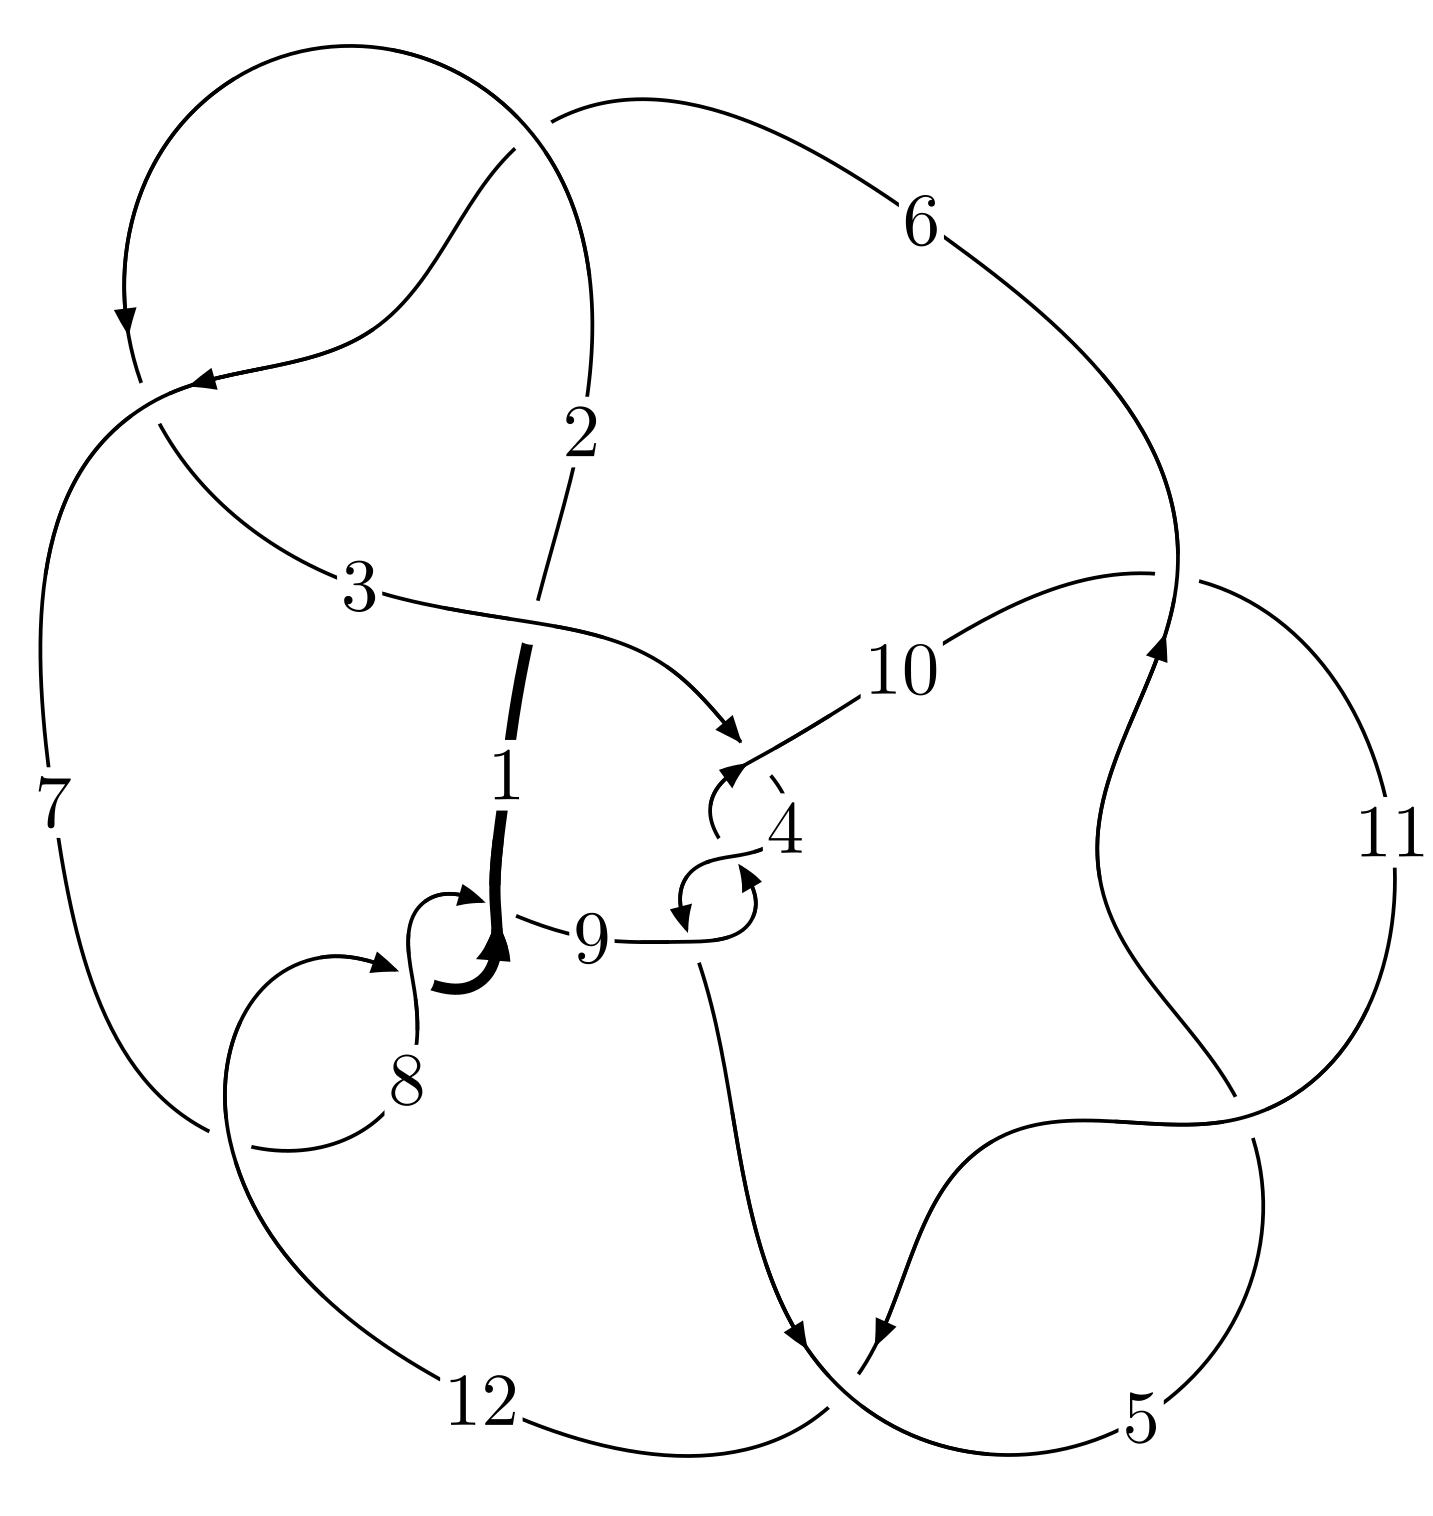
\includegraphics[width=112pt]{../../../GIT/diagram.site/Diagrams/png/1435_12a_0634.png}\\
\ \ \ A knot diagram\footnotemark}&
\allowdisplaybreaks
\textbf{Linearized knot diagam} \\
\cline{2-2}
 &
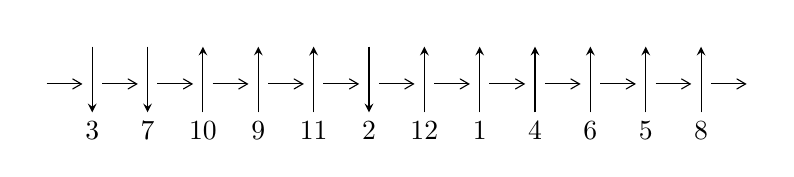
\begin{tikzpicture}[x=20pt, y=17pt]
	% nodes
	\node (C0) at (0, 0) {};
	\node (C1) at (1, 0) {};
	\node (C1U) at (1, +1) {};
	\node (C1D) at (1, -1) {3};

	\node (C2) at (2, 0) {};
	\node (C2U) at (2, +1) {};
	\node (C2D) at (2, -1) {7};

	\node (C3) at (3, 0) {};
	\node (C3U) at (3, +1) {};
	\node (C3D) at (3, -1) {10};

	\node (C4) at (4, 0) {};
	\node (C4U) at (4, +1) {};
	\node (C4D) at (4, -1) {9};

	\node (C5) at (5, 0) {};
	\node (C5U) at (5, +1) {};
	\node (C5D) at (5, -1) {11};

	\node (C6) at (6, 0) {};
	\node (C6U) at (6, +1) {};
	\node (C6D) at (6, -1) {2};

	\node (C7) at (7, 0) {};
	\node (C7U) at (7, +1) {};
	\node (C7D) at (7, -1) {12};

	\node (C8) at (8, 0) {};
	\node (C8U) at (8, +1) {};
	\node (C8D) at (8, -1) {1};

	\node (C9) at (9, 0) {};
	\node (C9U) at (9, +1) {};
	\node (C9D) at (9, -1) {4};

	\node (C10) at (10, 0) {};
	\node (C10U) at (10, +1) {};
	\node (C10D) at (10, -1) {6};

	\node (C11) at (11, 0) {};
	\node (C11U) at (11, +1) {};
	\node (C11D) at (11, -1) {5};

	\node (C12) at (12, 0) {};
	\node (C12U) at (12, +1) {};
	\node (C12D) at (12, -1) {8};
	\node (C13) at (13, 0) {};

	% arrows
	\draw[->,>={angle 60}]
	(C0) edge (C1) (C1) edge (C2) (C2) edge (C3) (C3) edge (C4) (C4) edge (C5) (C5) edge (C6) (C6) edge (C7) (C7) edge (C8) (C8) edge (C9) (C9) edge (C10) (C10) edge (C11) (C11) edge (C12) (C12) edge (C13) ;	\draw[->,>=stealth]
	(C1U) edge (C1D) (C2U) edge (C2D) (C3D) edge (C3U) (C4D) edge (C4U) (C5D) edge (C5U) (C6U) edge (C6D) (C7D) edge (C7U) (C8D) edge (C8U) (C9D) edge (C9U) (C10D) edge (C10U) (C11D) edge (C11U) (C12D) edge (C12U) ;
	\end{tikzpicture} \\
\hhline{~~} \\& 
\textbf{Solving Sequence} \\ \cline{2-2} 
 &
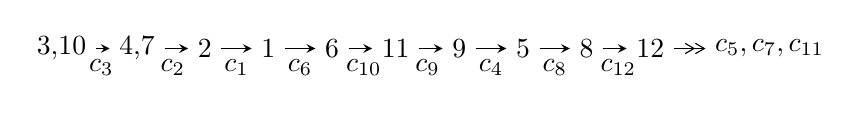
\begin{tikzpicture}[x=23pt, y=7pt]
	% node
	\node (A0) at (-1/8, 0) {3,10};
	\node (A1) at (17/16, 0) {4,7};
	\node (A2) at (17/8, 0) {2};
	\node (A3) at (25/8, 0) {1};
	\node (A4) at (33/8, 0) {6};
	\node (A5) at (41/8, 0) {11};
	\node (A6) at (49/8, 0) {9};
	\node (A7) at (57/8, 0) {5};
	\node (A8) at (65/8, 0) {8};
	\node (A9) at (73/8, 0) {12};
	\node (C1) at (1/2, -1) {$c_{3}$};
	\node (C2) at (13/8, -1) {$c_{2}$};
	\node (C3) at (21/8, -1) {$c_{1}$};
	\node (C4) at (29/8, -1) {$c_{6}$};
	\node (C5) at (37/8, -1) {$c_{10}$};
	\node (C6) at (45/8, -1) {$c_{9}$};
	\node (C7) at (53/8, -1) {$c_{4}$};
	\node (C8) at (61/8, -1) {$c_{8}$};
	\node (C9) at (69/8, -1) {$c_{12}$};
	\node (A10) at (11, 0) {$c_{5},c_{7},c_{11}$};

	% edge
	\draw[->,>=stealth]	
	(A0) edge (A1) (A1) edge (A2) (A2) edge (A3) (A3) edge (A4) (A4) edge (A5) (A5) edge (A6) (A6) edge (A7) (A7) edge (A8) (A8) edge (A9) ;
	\draw[->>,>={angle 60}]	
	(A9) edge (A10);
\end{tikzpicture} \\ 

\end{tabular} \\

\footnotetext{
The image of knot diagram is generated by the software ``\textbf{Draw programme}" developed by Andrew Bartholomew(\url{http://www.layer8.co.uk/maths/draw/index.htm\#Running-draw}), where we modified some parts for our purpose(\url{https://github.com/CATsTAILs/LinksPainter}).
}\phantom \\ \newline 
\centering \textbf{Ideals for irreducible components\footnotemark of $X_{\text{par}}$} 
 
\begin{align*}
I^u_{1}&=\langle 
-2 u^{24}-31 u^{22}+\cdots+16 b-6,\;- u^{24}+u^{23}+\cdots+32 a-22,\;u^{25}+15 u^{23}+\cdots-2 u-2\rangle \\
I^u_{2}&=\langle 
131149683608665 u^{33}-237748805942401 u^{32}+\cdots+4229403894019872 b-1000700151544160,\\
\phantom{I^u_{2}}&\phantom{= \langle  }218876053189111 u^{33}-464080060606921 u^{32}+\cdots+1409801298006624 a-1994609262976856,\\
\phantom{I^u_{2}}&\phantom{= \langle  }u^{34}-2 u^{33}+\cdots-36 u+8\rangle \\
I^u_{3}&=\langle 
- u^2 a+a u+u^2+b,\;-2 u^2 a+2 a^2+3 u^2-6 a+u+7,\;u^3+2 u-1\rangle \\
I^u_{4}&=\langle 
- u^2+b-1,\;a- u,\;u^3+2 u-1\rangle \\
I^u_{5}&=\langle 
a^3 u+a^3+3 a^2 u+2 a^2+3 a u+b+5 a+u+3,\;2 a^4+a^3 u+5 a^3-2 a^2 u+8 a^2-3 a u+5 a- u+1,\;u^2+1\rangle \\
I^u_{6}&=\langle 
-6 u^3 a^2-9 a^2 u^2+11 u^3 a+5 a^2 u-5 u^2 a+30 u^3+12 a^2-2 a u+2 u^2+43 b+21 a+18 u+26,\\
\phantom{I^u_{6}}&\phantom{= \langle  }2 u^3 a^2+2 u^3 a+a^3+2 a^2 u+u^2 a+4 u^3+2 a^2+a u- u^2+2 a+6 u,\;u^4+u^3+2 u^2+2 u+1\rangle \\
I^u_{7}&=\langle 
b-1,\;6 a+u-3,\;u^2+3\rangle \\
\\
I^v_{1}&=\langle 
a,\;b-1,\;v-1\rangle \\
\end{align*}
\raggedright * 8 irreducible components of $\dim_{\mathbb{C}}=0$, with total 91 representations.\\
\footnotetext{All coefficients of polynomials are rational numbers. But the coefficients are sometimes approximated in decimal forms when there is not enough margin.}
\newpage
\renewcommand{\arraystretch}{1}
\centering \section*{I. $I^u_{1}= \langle -2 u^{24}-31 u^{22}+\cdots+16 b-6,\;- u^{24}+u^{23}+\cdots+32 a-22,\;u^{25}+15 u^{23}+\cdots-2 u-2 \rangle$}
\flushleft \textbf{(i) Arc colorings}\\
\begin{tabular}{m{7pt} m{180pt} m{7pt} m{180pt} }
\flushright $a_{3}=$&$\begin{pmatrix}1\\0\end{pmatrix}$ \\
\flushright $a_{10}=$&$\begin{pmatrix}0\\u\end{pmatrix}$ \\
\flushright $a_{4}=$&$\begin{pmatrix}1\\- u^2\end{pmatrix}$ \\
\flushright $a_{7}=$&$\begin{pmatrix}\frac{1}{32} u^{24}-\frac{1}{32} u^{23}+\cdots+\frac{5}{4} u+\frac{11}{16}\\\frac{1}{8} u^{24}+\frac{31}{16} u^{22}+\cdots-\frac{3}{2} u+\frac{3}{8}\end{pmatrix}$ \\
\flushright $a_{2}=$&$\begin{pmatrix}\frac{1}{32} u^{24}-\frac{1}{32} u^{23}+\cdots+\frac{5}{4} u+\frac{11}{16}\\-\frac{3}{16} u^{24}+\frac{1}{8} u^{23}+\cdots+\frac{9}{8} u-\frac{7}{8}\end{pmatrix}$ \\
\flushright $a_{1}=$&$\begin{pmatrix}-0.156250 u^{24}+0.0937500 u^{23}+\cdots+2.37500 u-0.187500\\-\frac{3}{16} u^{24}+\frac{1}{8} u^{23}+\cdots+\frac{9}{8} u-\frac{7}{8}\end{pmatrix}$ \\
\flushright $a_{6}=$&$\begin{pmatrix}1\\\frac{1}{8} u^{23}+\frac{7}{4} u^{21}+\cdots-\frac{1}{4} u-\frac{1}{4}\end{pmatrix}$ \\
\flushright $a_{11}=$&$\begin{pmatrix}u\\\frac{1}{8} u^{24}+\frac{7}{4} u^{22}+\cdots-\frac{1}{4} u^2+\frac{3}{4} u\end{pmatrix}$ \\
\flushright $a_{9}=$&$\begin{pmatrix}- u\\u^3+u\end{pmatrix}$ \\
\flushright $a_{5}=$&$\begin{pmatrix}u^2+1\\- u^4-2 u^2\end{pmatrix}$ \\
\flushright $a_{8}=$&$\begin{pmatrix}\frac{1}{32} u^{24}-\frac{3}{32} u^{23}+\cdots-\frac{11}{8} u-\frac{1}{16}\\\frac{1}{16} u^{24}+\frac{1}{16} u^{23}+\cdots+\frac{1}{2} u-\frac{1}{8}\end{pmatrix}$ \\
\flushright $a_{12}=$&$\begin{pmatrix}u^3+2 u\\\frac{1}{8} u^{24}+\frac{7}{4} u^{22}+\cdots-\frac{1}{4} u^2+\frac{3}{4} u\end{pmatrix}$\\&\end{tabular}
\flushleft \textbf{(ii) Obstruction class $= -1$}\\~\\
\flushleft \textbf{(iii) Cusp Shapes $= \frac{7}{8} u^{24}+\frac{3}{8} u^{23}+\cdots+\frac{1}{2} u+\frac{7}{4}$}\\~\\
\newpage\renewcommand{\arraystretch}{1}
\flushleft \textbf{(iv) u-Polynomials at the component}\newline \\
\begin{tabular}{m{50pt}|m{274pt}}
Crossings & \hspace{64pt}u-Polynomials at each crossing \\
\hline $$\begin{aligned}c_{1}\end{aligned}$$&$\begin{aligned}
&u^{25}+10 u^{24}+\cdots+1455 u+169
\end{aligned}$\\
\hline $$\begin{aligned}c_{2},c_{6}\end{aligned}$$&$\begin{aligned}
&u^{25}-6 u^{24}+\cdots+57 u-13
\end{aligned}$\\
\hline $$\begin{aligned}c_{3},c_{4},c_{5}\\c_{9},c_{10},c_{11}\end{aligned}$$&$\begin{aligned}
&u^{25}+15 u^{23}+\cdots-2 u-2
\end{aligned}$\\
\hline $$\begin{aligned}c_{7},c_{8},c_{12}\end{aligned}$$&$\begin{aligned}
&u^{25}+6 u^{24}+\cdots-3 u-13
\end{aligned}$\\
\hline
\end{tabular}\\~\\
\newpage\renewcommand{\arraystretch}{1}
\flushleft \textbf{(v) Riley Polynomials at the component}\newline \\
\begin{tabular}{m{50pt}|m{274pt}}
Crossings & \hspace{64pt}Riley Polynomials at each crossing \\
\hline $$\begin{aligned}c_{1}\end{aligned}$$&$\begin{aligned}
&y^{25}+14 y^{24}+\cdots+367199 y-28561
\end{aligned}$\\
\hline $$\begin{aligned}c_{2},c_{6}\end{aligned}$$&$\begin{aligned}
&y^{25}-10 y^{24}+\cdots+1455 y-169
\end{aligned}$\\
\hline $$\begin{aligned}c_{3},c_{4},c_{5}\\c_{9},c_{10},c_{11}\end{aligned}$$&$\begin{aligned}
&y^{25}+30 y^{24}+\cdots-24 y-4
\end{aligned}$\\
\hline $$\begin{aligned}c_{7},c_{8},c_{12}\end{aligned}$$&$\begin{aligned}
&y^{25}-26 y^{24}+\cdots+191 y-169
\end{aligned}$\\
\hline
\end{tabular}\\~\\
\newpage\flushleft \textbf{(vi) Complex Volumes and Cusp Shapes}
$$\begin{array}{c|c|c}  
\text{Solutions to }I^u_{1}& \I (\text{vol} + \sqrt{-1}CS) & \text{Cusp shape}\\
 \hline 
\begin{aligned}
u &= \phantom{-}0.755535 + 0.415934 I \\
a &= -0.08824 - 1.55070 I \\
b &= -1.036580 + 0.642790 I\end{aligned}
 & \phantom{-}5.29214 + 6.95092 I & \phantom{-}9.63817 - 7.49283 I \\ \hline\begin{aligned}
u &= \phantom{-}0.755535 - 0.415934 I \\
a &= -0.08824 + 1.55070 I \\
b &= -1.036580 - 0.642790 I\end{aligned}
 & \phantom{-}5.29214 - 6.95092 I & \phantom{-}9.63817 + 7.49283 I \\ \hline\begin{aligned}
u &= -0.781688 + 0.222090 I \\
a &= \phantom{-}0.567778 - 0.932154 I \\
b &= -0.523390 + 0.782479 I\end{aligned}
 & \phantom{-}6.80658 - 1.60733 I & \phantom{-}12.68937 + 1.64186 I \\ \hline\begin{aligned}
u &= -0.781688 - 0.222090 I \\
a &= \phantom{-}0.567778 + 0.932154 I \\
b &= -0.523390 - 0.782479 I\end{aligned}
 & \phantom{-}6.80658 + 1.60733 I & \phantom{-}12.68937 - 1.64186 I \\ \hline\begin{aligned}
u &= \phantom{-}0.048749 + 1.304960 I \\
a &= \phantom{-}0.055343 - 0.974408 I \\
b &= -0.941899 + 1.022970 I\end{aligned}
 & \phantom{-}1.65681 + 3.64991 I & \phantom{-}0.77498 - 3.11405 I \\ \hline\begin{aligned}
u &= \phantom{-}0.048749 - 1.304960 I \\
a &= \phantom{-}0.055343 + 0.974408 I \\
b &= -0.941899 - 1.022970 I\end{aligned}
 & \phantom{-}1.65681 - 3.64991 I & \phantom{-}0.77498 + 3.11405 I \\ \hline\begin{aligned}
u &= \phantom{-}0.071780 + 0.652870 I \\
a &= \phantom{-}0.451606 - 0.184043 I \\
b &= \phantom{-}0.898942 + 0.773875 I\end{aligned}
 & \phantom{-}4.71249 - 2.92993 I & \phantom{-}11.02910 + 1.21081 I \\ \hline\begin{aligned}
u &= \phantom{-}0.071780 - 0.652870 I \\
a &= \phantom{-}0.451606 + 0.184043 I \\
b &= \phantom{-}0.898942 - 0.773875 I\end{aligned}
 & \phantom{-}4.71249 + 2.92993 I & \phantom{-}11.02910 - 1.21081 I \\ \hline\begin{aligned}
u &= -0.570291 + 0.288945 I \\
a &= \phantom{-}0.18281 + 2.07363 I \\
b &= -0.957814 - 0.478527 I\end{aligned}
 & -0.33137 - 3.73744 I & \phantom{-}6.36857 + 8.33061 I \\ \hline\begin{aligned}
u &= -0.570291 - 0.288945 I \\
a &= \phantom{-}0.18281 - 2.07363 I \\
b &= -0.957814 + 0.478527 I\end{aligned}
 & -0.33137 + 3.73744 I & \phantom{-}6.36857 - 8.33061 I\\
 \hline 
 \end{array}$$\newpage$$\begin{array}{c|c|c}  
\text{Solutions to }I^u_{1}& \I (\text{vol} + \sqrt{-1}CS) & \text{Cusp shape}\\
 \hline 
\begin{aligned}
u &= \phantom{-}0.09300 + 1.43892 I \\
a &= \phantom{-}0.448195 + 0.914529 I \\
b &= -0.567898 - 0.881693 I\end{aligned}
 & -7.75327 - 0.62404 I & \phantom{-}1.11905 + 1.82325 I \\ \hline\begin{aligned}
u &= \phantom{-}0.09300 - 1.43892 I \\
a &= \phantom{-}0.448195 - 0.914529 I \\
b &= -0.567898 + 0.881693 I\end{aligned}
 & -7.75327 + 0.62404 I & \phantom{-}1.11905 - 1.82325 I \\ \hline\begin{aligned}
u &= \phantom{-}0.34989 + 1.44000 I \\
a &= \phantom{-}0.447471 + 0.624414 I \\
b &= -0.241733 - 1.058110 I\end{aligned}
 & -3.68401 + 9.94366 I & \phantom{-}4.37752 - 5.16617 I \\ \hline\begin{aligned}
u &= \phantom{-}0.34989 - 1.44000 I \\
a &= \phantom{-}0.447471 - 0.624414 I \\
b &= -0.241733 + 1.058110 I\end{aligned}
 & -3.68401 - 9.94366 I & \phantom{-}4.37752 + 5.16617 I \\ \hline\begin{aligned}
u &= \phantom{-}0.32103 + 1.50150 I \\
a &= -0.46525 - 1.45818 I \\
b &= -1.198590 + 0.622421 I\end{aligned}
 & -12.0801 + 10.8715 I & -1.24061 - 6.62726 I \\ \hline\begin{aligned}
u &= \phantom{-}0.32103 - 1.50150 I \\
a &= -0.46525 + 1.45818 I \\
b &= -1.198590 - 0.622421 I\end{aligned}
 & -12.0801 - 10.8715 I & -1.24061 + 6.62726 I \\ \hline\begin{aligned}
u &= -0.40263 + 1.50474 I \\
a &= -0.57474 + 1.36291 I \\
b &= -1.262700 - 0.622947 I\end{aligned}
 & -6.8511 - 15.9422 I & \phantom{-}2.15332 + 8.18122 I \\ \hline\begin{aligned}
u &= -0.40263 - 1.50474 I \\
a &= -0.57474 - 1.36291 I \\
b &= -1.262700 + 0.622947 I\end{aligned}
 & -6.8511 + 15.9422 I & \phantom{-}2.15332 - 8.18122 I \\ \hline\begin{aligned}
u &= -0.116143 + 0.395232 I \\
a &= \phantom{-}0.523724 + 0.083480 I \\
b &= \phantom{-}0.862091 - 0.296810 I\end{aligned}
 & -1.35428 + 1.12969 I & \phantom{-}0.98953 - 1.48650 I \\ \hline\begin{aligned}
u &= -0.116143 - 0.395232 I \\
a &= \phantom{-}0.523724 - 0.083480 I \\
b &= \phantom{-}0.862091 + 0.296810 I\end{aligned}
 & -1.35428 - 1.12969 I & \phantom{-}0.98953 + 1.48650 I\\
 \hline 
 \end{array}$$\newpage$$\begin{array}{c|c|c}  
\text{Solutions to }I^u_{1}& \I (\text{vol} + \sqrt{-1}CS) & \text{Cusp shape}\\
 \hline 
\begin{aligned}
u &= \phantom{-}0.13068 + 1.60153 I \\
a &= \phantom{-}0.436301 - 0.037125 I \\
b &= \phantom{-}1.275520 + 0.193623 I\end{aligned}
 & -15.0829 + 1.6460 I & -4.49592 - 1.15064 I \\ \hline\begin{aligned}
u &= \phantom{-}0.13068 - 1.60153 I \\
a &= \phantom{-}0.436301 + 0.037125 I \\
b &= \phantom{-}1.275520 - 0.193623 I\end{aligned}
 & -15.0829 - 1.6460 I & -4.49592 + 1.15064 I \\ \hline\begin{aligned}
u &= \phantom{-}0.369219\phantom{ +0.000000I} \\
a &= \phantom{-}2.02103\phantom{ +0.000000I} \\
b &= -0.505202\phantom{ +0.000000I}\end{aligned}
 & \phantom{-}0.738512\phantom{ +0.000000I} & \phantom{-}14.6480\phantom{ +0.000000I} \\ \hline\begin{aligned}
u &= -0.08452 + 1.78825 I \\
a &= \phantom{-}0.504494 + 0.068165 I \\
b &= \phantom{-}0.946646 - 0.263021 I\end{aligned}
 & -12.82360 + 1.06304 I & \phantom{-}4.27303 - 7.22736 I \\ \hline\begin{aligned}
u &= -0.08452 - 1.78825 I \\
a &= \phantom{-}0.504494 - 0.068165 I \\
b &= \phantom{-}0.946646 + 0.263021 I\end{aligned}
 & -12.82360 - 1.06304 I & \phantom{-}4.27303 + 7.22736 I\\
 \hline 
 \end{array}$$\newpage\newpage\renewcommand{\arraystretch}{1}
\centering \section*{II. $I^u_{2}= \langle 1.31\times10^{14} u^{33}-2.38\times10^{14} u^{32}+\cdots+4.23\times10^{15} b-1.00\times10^{15},\;2.19\times10^{14} u^{33}-4.64\times10^{14} u^{32}+\cdots+1.41\times10^{15} a-1.99\times10^{15},\;u^{34}-2 u^{33}+\cdots-36 u+8 \rangle$}
\flushleft \textbf{(i) Arc colorings}\\
\begin{tabular}{m{7pt} m{180pt} m{7pt} m{180pt} }
\flushright $a_{3}=$&$\begin{pmatrix}1\\0\end{pmatrix}$ \\
\flushright $a_{10}=$&$\begin{pmatrix}0\\u\end{pmatrix}$ \\
\flushright $a_{4}=$&$\begin{pmatrix}1\\- u^2\end{pmatrix}$ \\
\flushright $a_{7}=$&$\begin{pmatrix}-0.155253 u^{33}+0.329181 u^{32}+\cdots-29.1112 u+1.41482\\-0.0310090 u^{33}+0.0562133 u^{32}+\cdots+2.78205 u+0.236605\end{pmatrix}$ \\
\flushright $a_{2}=$&$\begin{pmatrix}0.0670221 u^{33}-0.211355 u^{32}+\cdots+28.1192 u-2.65059\\-0.0233286 u^{33}+0.0485749 u^{32}+\cdots-3.94112 u+0.296004\end{pmatrix}$ \\
\flushright $a_{1}=$&$\begin{pmatrix}0.0436936 u^{33}-0.162780 u^{32}+\cdots+24.1780 u-2.35459\\-0.0233286 u^{33}+0.0485749 u^{32}+\cdots-3.94112 u+0.296004\end{pmatrix}$ \\
\flushright $a_{6}=$&$\begin{pmatrix}-0.164018 u^{33}+0.329267 u^{32}+\cdots-9.73795 u-1.66269\\-0.0499240 u^{33}+0.0898833 u^{32}+\cdots-1.35647 u+1.00985\end{pmatrix}$ \\
\flushright $a_{11}=$&$\begin{pmatrix}0.123769 u^{33}-0.297461 u^{32}+\cdots+33.8173 u-5.81214\\0.0111960 u^{33}+0.0150363 u^{32}+\cdots-3.77992 u+0.912751\end{pmatrix}$ \\
\flushright $a_{9}=$&$\begin{pmatrix}- u\\u^3+u\end{pmatrix}$ \\
\flushright $a_{5}=$&$\begin{pmatrix}u^2+1\\- u^4-2 u^2\end{pmatrix}$ \\
\flushright $a_{8}=$&$\begin{pmatrix}0.173662 u^{33}-0.284141 u^{32}+\cdots+14.3998 u-0.525050\\-0.00389825 u^{33}+0.0271836 u^{32}+\cdots-1.92616 u+0.497794\end{pmatrix}$ \\
\flushright $a_{12}=$&$\begin{pmatrix}0.134965 u^{33}-0.282425 u^{32}+\cdots+28.0374 u-4.89939\\-0.0361733 u^{33}+0.110465 u^{32}+\cdots-6.82518 u+1.61157\end{pmatrix}$\\&\end{tabular}
\flushleft \textbf{(ii) Obstruction class $= -1$}\\~\\
\flushleft \textbf{(iii) Cusp Shapes $= -\frac{11998428764201}{44056290562707} u^{33}+\frac{35190412311283}{88112581125414} u^{32}+\cdots+\frac{1450723211244922}{44056290562707} u+\frac{103896439660429}{44056290562707}$}\\~\\
\newpage\renewcommand{\arraystretch}{1}
\flushleft \textbf{(iv) u-Polynomials at the component}\newline \\
\begin{tabular}{m{50pt}|m{274pt}}
Crossings & \hspace{64pt}u-Polynomials at each crossing \\
\hline $$\begin{aligned}c_{1}\end{aligned}$$&$\begin{aligned}
&(u^{17}+8 u^{16}+\cdots+3 u+1)^{2}
\end{aligned}$\\
\hline $$\begin{aligned}c_{2},c_{6}\end{aligned}$$&$\begin{aligned}
&(u^{17}+2 u^{16}+\cdots- u-1)^{2}
\end{aligned}$\\
\hline $$\begin{aligned}c_{3},c_{4},c_{5}\\c_{9},c_{10},c_{11}\end{aligned}$$&$\begin{aligned}
&u^{34}-2 u^{33}+\cdots-36 u+8
\end{aligned}$\\
\hline $$\begin{aligned}c_{7},c_{8},c_{12}\end{aligned}$$&$\begin{aligned}
&(u^{17}-2 u^{16}+\cdots+3 u-1)^{2}
\end{aligned}$\\
\hline
\end{tabular}\\~\\
\newpage\renewcommand{\arraystretch}{1}
\flushleft \textbf{(v) Riley Polynomials at the component}\newline \\
\begin{tabular}{m{50pt}|m{274pt}}
Crossings & \hspace{64pt}Riley Polynomials at each crossing \\
\hline $$\begin{aligned}c_{1}\end{aligned}$$&$\begin{aligned}
&(y^{17}+4 y^{16}+\cdots-13 y-1)^{2}
\end{aligned}$\\
\hline $$\begin{aligned}c_{2},c_{6}\end{aligned}$$&$\begin{aligned}
&(y^{17}-8 y^{16}+\cdots+3 y-1)^{2}
\end{aligned}$\\
\hline $$\begin{aligned}c_{3},c_{4},c_{5}\\c_{9},c_{10},c_{11}\end{aligned}$$&$\begin{aligned}
&y^{34}+28 y^{33}+\cdots+2192 y+64
\end{aligned}$\\
\hline $$\begin{aligned}c_{7},c_{8},c_{12}\end{aligned}$$&$\begin{aligned}
&(y^{17}-16 y^{16}+\cdots+19 y-1)^{2}
\end{aligned}$\\
\hline
\end{tabular}\\~\\
\newpage\flushleft \textbf{(vi) Complex Volumes and Cusp Shapes}
$$\begin{array}{c|c|c}  
\text{Solutions to }I^u_{2}& \I (\text{vol} + \sqrt{-1}CS) & \text{Cusp shape}\\
 \hline 
\begin{aligned}
u &= \phantom{-}0.864072 + 0.421442 I \\
a &= -0.60307 + 1.70997 I \\
b &= \phantom{-}1.130680 - 0.513073 I\end{aligned}
 & -5.86965 + 6.57063 I & \phantom{-}0.73995 - 6.43452 I \\ \hline\begin{aligned}
u &= \phantom{-}0.864072 - 0.421442 I \\
a &= -0.60307 - 1.70997 I \\
b &= \phantom{-}1.130680 + 0.513073 I\end{aligned}
 & -5.86965 - 6.57063 I & \phantom{-}0.73995 + 6.43452 I \\ \hline\begin{aligned}
u &= \phantom{-}0.701574 + 0.772236 I \\
a &= \phantom{-}0.671036 + 0.299184 I \\
b &= -1.128570 - 0.359117 I\end{aligned}
 & -6.94910 - 1.22724 I & -2.14847 + 0.85505 I \\ \hline\begin{aligned}
u &= \phantom{-}0.701574 - 0.772236 I \\
a &= \phantom{-}0.671036 - 0.299184 I \\
b &= -1.128570 + 0.359117 I\end{aligned}
 & -6.94910 + 1.22724 I & -2.14847 - 0.85505 I \\ \hline\begin{aligned}
u &= -0.400299 + 0.849296 I \\
a &= \phantom{-}0.488205 - 0.936880 I \\
b &= \phantom{-}0.796399 + 0.723427 I\end{aligned}
 & \phantom{-}4.74481 - 2.71165 I & \phantom{-}9.84242 + 3.13710 I \\ \hline\begin{aligned}
u &= -0.400299 - 0.849296 I \\
a &= \phantom{-}0.488205 + 0.936880 I \\
b &= \phantom{-}0.796399 - 0.723427 I\end{aligned}
 & \phantom{-}4.74481 + 2.71165 I & \phantom{-}9.84242 - 3.13710 I \\ \hline\begin{aligned}
u &= -1.015190 + 0.363118 I \\
a &= -0.42443 - 1.39736 I \\
b &= \phantom{-}1.172120 + 0.583556 I\end{aligned}
 & -0.88663 - 10.83370 I & \phantom{-}4.89378 + 7.41261 I \\ \hline\begin{aligned}
u &= -1.015190 - 0.363118 I \\
a &= -0.42443 + 1.39736 I \\
b &= \phantom{-}1.172120 - 0.583556 I\end{aligned}
 & -0.88663 + 10.83370 I & \phantom{-}4.89378 - 7.41261 I \\ \hline\begin{aligned}
u &= \phantom{-}0.882304 + 0.259295 I \\
a &= -0.201550 - 1.387080 I \\
b &= \phantom{-}0.288739 + 0.863831 I\end{aligned}
 & \phantom{-}1.75994 + 5.51158 I & \phantom{-}8.25126 - 3.84490 I \\ \hline\begin{aligned}
u &= \phantom{-}0.882304 - 0.259295 I \\
a &= -0.201550 + 1.387080 I \\
b &= \phantom{-}0.288739 - 0.863831 I\end{aligned}
 & \phantom{-}1.75994 - 5.51158 I & \phantom{-}8.25126 + 3.84490 I\\
 \hline 
 \end{array}$$\newpage$$\begin{array}{c|c|c}  
\text{Solutions to }I^u_{2}& \I (\text{vol} + \sqrt{-1}CS) & \text{Cusp shape}\\
 \hline 
\begin{aligned}
u &= -0.231948 + 1.077680 I \\
a &= -0.17884 + 1.65758 I \\
b &= -0.867068\phantom{ +0.000000I}\end{aligned}
 & -4.54799\phantom{ +0.000000I} & -4.68792 + 0. I\phantom{ +0.000000I} \\ \hline\begin{aligned}
u &= -0.231948 - 1.077680 I \\
a &= -0.17884 - 1.65758 I \\
b &= -0.867068\phantom{ +0.000000I}\end{aligned}
 & -4.54799\phantom{ +0.000000I} & -4.68792 + 0. I\phantom{ +0.000000I} \\ \hline\begin{aligned}
u &= -0.001691 + 1.105180 I \\
a &= -0.516445 + 0.866608 I \\
b &= \phantom{-}0.621791 - 0.419413 I\end{aligned}
 & -1.98005 + 1.46955 I & \phantom{-}7.63583 - 4.66528 I \\ \hline\begin{aligned}
u &= -0.001691 - 1.105180 I \\
a &= -0.516445 - 0.866608 I \\
b &= \phantom{-}0.621791 + 0.419413 I\end{aligned}
 & -1.98005 - 1.46955 I & \phantom{-}7.63583 + 4.66528 I \\ \hline\begin{aligned}
u &= \phantom{-}0.553439 + 1.087560 I \\
a &= -0.737070 - 0.832523 I \\
b &= -0.374678 + 0.520641 I\end{aligned}
 & -0.670307 - 0.433874 I & \phantom{-}6.56834 - 0.87540 I \\ \hline\begin{aligned}
u &= \phantom{-}0.553439 - 1.087560 I \\
a &= -0.737070 + 0.832523 I \\
b &= -0.374678 - 0.520641 I\end{aligned}
 & -0.670307 + 0.433874 I & \phantom{-}6.56834 + 0.87540 I \\ \hline\begin{aligned}
u &= -0.815743 + 0.977729 I \\
a &= \phantom{-}0.365441 - 0.177204 I \\
b &= -1.072950 + 0.498433 I\end{aligned}
 & -2.67943 + 4.64771 I & \phantom{-}3.56085 - 4.11695 I \\ \hline\begin{aligned}
u &= -0.815743 - 0.977729 I \\
a &= \phantom{-}0.365441 + 0.177204 I \\
b &= -1.072950 - 0.498433 I\end{aligned}
 & -2.67943 - 4.64771 I & \phantom{-}3.56085 + 4.11695 I \\ \hline\begin{aligned}
u &= \phantom{-}0.510396 + 0.397212 I \\
a &= -0.577773 + 0.030688 I \\
b &= \phantom{-}0.796399 + 0.723427 I\end{aligned}
 & \phantom{-}4.74481 - 2.71165 I & \phantom{-}9.84242 + 3.13710 I \\ \hline\begin{aligned}
u &= \phantom{-}0.510396 - 0.397212 I \\
a &= -0.577773 - 0.030688 I \\
b &= \phantom{-}0.796399 - 0.723427 I\end{aligned}
 & \phantom{-}4.74481 + 2.71165 I & \phantom{-}9.84242 - 3.13710 I\\
 \hline 
 \end{array}$$\newpage$$\begin{array}{c|c|c}  
\text{Solutions to }I^u_{2}& \I (\text{vol} + \sqrt{-1}CS) & \text{Cusp shape}\\
 \hline 
\begin{aligned}
u &= \phantom{-}0.281426 + 1.352580 I \\
a &= -0.239793 - 0.110964 I \\
b &= -0.374678 - 0.520641 I\end{aligned}
 & -0.670307 + 0.433874 I & \phantom{-}6.56834 + 0.87540 I \\ \hline\begin{aligned}
u &= \phantom{-}0.281426 - 1.352580 I \\
a &= -0.239793 + 0.110964 I \\
b &= -0.374678 + 0.520641 I\end{aligned}
 & -0.670307 - 0.433874 I & \phantom{-}6.56834 - 0.87540 I \\ \hline\begin{aligned}
u &= -0.303439 + 1.375590 I \\
a &= -0.284613 + 0.260893 I \\
b &= \phantom{-}0.288739 - 0.863831 I\end{aligned}
 & \phantom{-}1.75994 - 5.51158 I & \phantom{-}8.25126 + 3.84490 I \\ \hline\begin{aligned}
u &= -0.303439 - 1.375590 I \\
a &= -0.284613 - 0.260893 I \\
b &= \phantom{-}0.288739 + 0.863831 I\end{aligned}
 & \phantom{-}1.75994 + 5.51158 I & \phantom{-}8.25126 - 3.84490 I \\ \hline\begin{aligned}
u &= \phantom{-}0.04104 + 1.42314 I \\
a &= -1.165140 - 0.532963 I \\
b &= -1.128570 + 0.359117 I\end{aligned}
 & -6.94910 + 1.22724 I & -2.14847 - 0.85505 I \\ \hline\begin{aligned}
u &= \phantom{-}0.04104 - 1.42314 I \\
a &= -1.165140 + 0.532963 I \\
b &= -1.128570 - 0.359117 I\end{aligned}
 & -6.94910 - 1.22724 I & -2.14847 + 0.85505 I \\ \hline\begin{aligned}
u &= -0.20733 + 1.42614 I \\
a &= \phantom{-}0.93419 - 1.28605 I \\
b &= \phantom{-}1.130680 + 0.513073 I\end{aligned}
 & -5.86965 - 6.57063 I & \phantom{-}0.73995 + 6.43452 I \\ \hline\begin{aligned}
u &= -0.20733 - 1.42614 I \\
a &= \phantom{-}0.93419 + 1.28605 I \\
b &= \phantom{-}1.130680 - 0.513073 I\end{aligned}
 & -5.86965 + 6.57063 I & \phantom{-}0.73995 - 6.43452 I \\ \hline\begin{aligned}
u &= \phantom{-}0.29669 + 1.49249 I \\
a &= \phantom{-}0.89771 + 1.10113 I \\
b &= \phantom{-}1.172120 - 0.583556 I\end{aligned}
 & -0.88663 + 10.83370 I & \phantom{-}4.89378 - 7.41261 I \\ \hline\begin{aligned}
u &= \phantom{-}0.29669 - 1.49249 I \\
a &= \phantom{-}0.89771 - 1.10113 I \\
b &= \phantom{-}1.172120 + 0.583556 I\end{aligned}
 & -0.88663 - 10.83370 I & \phantom{-}4.89378 + 7.41261 I\\
 \hline 
 \end{array}$$\newpage$$\begin{array}{c|c|c}  
\text{Solutions to }I^u_{2}& \I (\text{vol} + \sqrt{-1}CS) & \text{Cusp shape}\\
 \hline 
\begin{aligned}
u &= -0.16100 + 1.54040 I \\
a &= -0.966662 + 0.555173 I \\
b &= -1.072950 - 0.498433 I\end{aligned}
 & -2.67943 - 4.64771 I & \phantom{-}3.56085 + 4.11695 I \\ \hline\begin{aligned}
u &= -0.16100 - 1.54040 I \\
a &= -0.966662 - 0.555173 I \\
b &= -1.072950 + 0.498433 I\end{aligned}
 & -2.67943 + 4.64771 I & \phantom{-}3.56085 - 4.11695 I \\ \hline\begin{aligned}
u &= \phantom{-}0.005683 + 0.262839 I \\
a &= -3.96119 - 3.25601 I \\
b &= \phantom{-}0.621791 + 0.419413 I\end{aligned}
 & -1.98005 - 1.46955 I & \phantom{-}7.63583 + 4.66528 I \\ \hline\begin{aligned}
u &= \phantom{-}0.005683 - 0.262839 I \\
a &= -3.96119 + 3.25601 I \\
b &= \phantom{-}0.621791 - 0.419413 I\end{aligned}
 & -1.98005 + 1.46955 I & \phantom{-}7.63583 - 4.66528 I\\
 \hline 
 \end{array}$$\newpage\newpage\renewcommand{\arraystretch}{1}
\centering \section*{III. $I^u_{3}= \langle - u^2 a+a u+u^2+b,\;-2 u^2 a+2 a^2+3 u^2-6 a+u+7,\;u^3+2 u-1 \rangle$}
\flushleft \textbf{(i) Arc colorings}\\
\begin{tabular}{m{7pt} m{180pt} m{7pt} m{180pt} }
\flushright $a_{3}=$&$\begin{pmatrix}1\\0\end{pmatrix}$ \\
\flushright $a_{10}=$&$\begin{pmatrix}0\\u\end{pmatrix}$ \\
\flushright $a_{4}=$&$\begin{pmatrix}1\\- u^2\end{pmatrix}$ \\
\flushright $a_{7}=$&$\begin{pmatrix}a\\u^2 a- a u- u^2\end{pmatrix}$ \\
\flushright $a_{2}=$&$\begin{pmatrix}a\\- u^2 a+2 a u+u^2- a\end{pmatrix}$ \\
\flushright $a_{1}=$&$\begin{pmatrix}- u^2 a+2 a u+u^2\\- u^2 a+2 a u+u^2- a\end{pmatrix}$ \\
\flushright $a_{6}=$&$\begin{pmatrix}1\\u-1\end{pmatrix}$ \\
\flushright $a_{11}=$&$\begin{pmatrix}u\\u^2\end{pmatrix}$ \\
\flushright $a_{9}=$&$\begin{pmatrix}- u\\- u+1\end{pmatrix}$ \\
\flushright $a_{5}=$&$\begin{pmatrix}u^2+1\\- u\end{pmatrix}$ \\
\flushright $a_{8}=$&$\begin{pmatrix}- u^2 a+a u+u^2- a\\- u^2 a+a u+u^2\end{pmatrix}$ \\
\flushright $a_{12}=$&$\begin{pmatrix}1\\0\end{pmatrix}$\\&\end{tabular}
\flushleft \textbf{(ii) Obstruction class $= -1$}\\~\\
\flushleft \textbf{(iii) Cusp Shapes $= 4 u^2+4 u+10$}\\~\\
\newpage\renewcommand{\arraystretch}{1}
\flushleft \textbf{(iv) u-Polynomials at the component}\newline \\
\begin{tabular}{m{50pt}|m{274pt}}
Crossings & \hspace{64pt}u-Polynomials at each crossing \\
\hline $$\begin{aligned}c_{1}\end{aligned}$$&$\begin{aligned}
&u^6+3 u^5+u^4-3 u^3+3 u^2+2 u+1
\end{aligned}$\\
\hline $$\begin{aligned}c_{2},c_{6},c_{7}\\c_{8},c_{12}\end{aligned}$$&$\begin{aligned}
&u^6+u^5- u^4+u^3+u^2-2 u+1
\end{aligned}$\\
\hline $$\begin{aligned}c_{3},c_{4},c_{5}\\c_{9},c_{10},c_{11}\end{aligned}$$&$\begin{aligned}
&(u^3+2 u-1)^2
\end{aligned}$\\
\hline
\end{tabular}\\~\\
\newpage\renewcommand{\arraystretch}{1}
\flushleft \textbf{(v) Riley Polynomials at the component}\newline \\
\begin{tabular}{m{50pt}|m{274pt}}
Crossings & \hspace{64pt}Riley Polynomials at each crossing \\
\hline $$\begin{aligned}c_{1}\end{aligned}$$&$\begin{aligned}
&y^6-7 y^5+25 y^4-13 y^3+23 y^2+2 y+1
\end{aligned}$\\
\hline $$\begin{aligned}c_{2},c_{6},c_{7}\\c_{8},c_{12}\end{aligned}$$&$\begin{aligned}
&y^6-3 y^5+y^4+3 y^3+3 y^2-2 y+1
\end{aligned}$\\
\hline $$\begin{aligned}c_{3},c_{4},c_{5}\\c_{9},c_{10},c_{11}\end{aligned}$$&$\begin{aligned}
&(y^3+4 y^2+4 y-1)^2
\end{aligned}$\\
\hline
\end{tabular}\\~\\
\newpage\flushleft \textbf{(vi) Complex Volumes and Cusp Shapes}
$$\begin{array}{c|c|c}  
\text{Solutions to }I^u_{3}& \I (\text{vol} + \sqrt{-1}CS) & \text{Cusp shape}\\
 \hline 
\begin{aligned}
u &= -0.22670 + 1.46771 I \\
a &= \phantom{-}0.493675 - 0.712154 I \\
b &= -0.342537 + 0.948428 I\end{aligned}
 & -9.44074 - 5.13794 I & \phantom{-}0.68207 + 3.20902 I \\ \hline\begin{aligned}
u &= -0.22670 + 1.46771 I \\
a &= \phantom{-}0.403540 + 0.046697 I \\
b &= \phantom{-}1.44532 - 0.28297 I\end{aligned}
 & -9.44074 - 5.13794 I & \phantom{-}0.68207 + 3.20902 I \\ \hline\begin{aligned}
u &= -0.22670 - 1.46771 I \\
a &= \phantom{-}0.493675 + 0.712154 I \\
b &= -0.342537 - 0.948428 I\end{aligned}
 & -9.44074 + 5.13794 I & \phantom{-}0.68207 - 3.20902 I \\ \hline\begin{aligned}
u &= -0.22670 - 1.46771 I \\
a &= \phantom{-}0.403540 - 0.046697 I \\
b &= \phantom{-}1.44532 + 0.28297 I\end{aligned}
 & -9.44074 + 5.13794 I & \phantom{-}0.68207 - 3.20902 I \\ \hline\begin{aligned}
u &= \phantom{-}0.453398\phantom{ +0.000000I} \\
a &= \phantom{-}1.60278 + 1.21084 I \\
b &= -0.602785 - 0.300080 I\end{aligned}
 & \phantom{-}0.787199\phantom{ +0.000000I} & \phantom{-}12.6360\phantom{ +0.000000I} \\ \hline\begin{aligned}
u &= \phantom{-}0.453398\phantom{ +0.000000I} \\
a &= \phantom{-}1.60278 - 1.21084 I \\
b &= -0.602785 + 0.300080 I\end{aligned}
 & \phantom{-}0.787199\phantom{ +0.000000I} & \phantom{-}12.6360\phantom{ +0.000000I}\\
 \hline 
 \end{array}$$\newpage\newpage\renewcommand{\arraystretch}{1}
\centering \section*{IV. $I^u_{4}= \langle - u^2+b-1,\;a- u,\;u^3+2 u-1 \rangle$}
\flushleft \textbf{(i) Arc colorings}\\
\begin{tabular}{m{7pt} m{180pt} m{7pt} m{180pt} }
\flushright $a_{3}=$&$\begin{pmatrix}1\\0\end{pmatrix}$ \\
\flushright $a_{10}=$&$\begin{pmatrix}0\\u\end{pmatrix}$ \\
\flushright $a_{4}=$&$\begin{pmatrix}1\\- u^2\end{pmatrix}$ \\
\flushright $a_{7}=$&$\begin{pmatrix}u\\u^2+1\end{pmatrix}$ \\
\flushright $a_{2}=$&$\begin{pmatrix}u\\- u-1\end{pmatrix}$ \\
\flushright $a_{1}=$&$\begin{pmatrix}-1\\- u-1\end{pmatrix}$ \\
\flushright $a_{6}=$&$\begin{pmatrix}1\\u-1\end{pmatrix}$ \\
\flushright $a_{11}=$&$\begin{pmatrix}u\\u^2\end{pmatrix}$ \\
\flushright $a_{9}=$&$\begin{pmatrix}- u\\- u+1\end{pmatrix}$ \\
\flushright $a_{5}=$&$\begin{pmatrix}u^2+1\\- u\end{pmatrix}$ \\
\flushright $a_{8}=$&$\begin{pmatrix}- u^2- u-1\\- u^2-1\end{pmatrix}$ \\
\flushright $a_{12}=$&$\begin{pmatrix}1\\0\end{pmatrix}$\\&\end{tabular}
\flushleft \textbf{(ii) Obstruction class $= -1$}\\~\\
\flushleft \textbf{(iii) Cusp Shapes $= 4 u^2+4 u+10$}\\~\\
\newpage\renewcommand{\arraystretch}{1}
\flushleft \textbf{(iv) u-Polynomials at the component}\newline \\
\begin{tabular}{m{50pt}|m{274pt}}
Crossings & \hspace{64pt}u-Polynomials at each crossing \\
\hline $$\begin{aligned}c_{1}\end{aligned}$$&$\begin{aligned}
&u^3+3 u^2+5 u+4
\end{aligned}$\\
\hline $$\begin{aligned}c_{2},c_{6},c_{7}\\c_{8},c_{12}\end{aligned}$$&$\begin{aligned}
&u^3- u^2- u+2
\end{aligned}$\\
\hline $$\begin{aligned}c_{3},c_{4},c_{5}\\c_{9},c_{10},c_{11}\end{aligned}$$&$\begin{aligned}
&u^3+2 u-1
\end{aligned}$\\
\hline
\end{tabular}\\~\\
\newpage\renewcommand{\arraystretch}{1}
\flushleft \textbf{(v) Riley Polynomials at the component}\newline \\
\begin{tabular}{m{50pt}|m{274pt}}
Crossings & \hspace{64pt}Riley Polynomials at each crossing \\
\hline $$\begin{aligned}c_{1}\end{aligned}$$&$\begin{aligned}
&y^3+y^2+y-16
\end{aligned}$\\
\hline $$\begin{aligned}c_{2},c_{6},c_{7}\\c_{8},c_{12}\end{aligned}$$&$\begin{aligned}
&y^3-3 y^2+5 y-4
\end{aligned}$\\
\hline $$\begin{aligned}c_{3},c_{4},c_{5}\\c_{9},c_{10},c_{11}\end{aligned}$$&$\begin{aligned}
&y^3+4 y^2+4 y-1
\end{aligned}$\\
\hline
\end{tabular}\\~\\
\newpage\flushleft \textbf{(vi) Complex Volumes and Cusp Shapes}
$$\begin{array}{c|c|c}  
\text{Solutions to }I^u_{4}& \I (\text{vol} + \sqrt{-1}CS) & \text{Cusp shape}\\
 \hline 
\begin{aligned}
u &= -0.22670 + 1.46771 I \\
a &= -0.22670 + 1.46771 I \\
b &= -1.102790 - 0.665457 I\end{aligned}
 & -9.44074 - 5.13794 I & \phantom{-}0.68207 + 3.20902 I \\ \hline\begin{aligned}
u &= -0.22670 - 1.46771 I \\
a &= -0.22670 - 1.46771 I \\
b &= -1.102790 + 0.665457 I\end{aligned}
 & -9.44074 + 5.13794 I & \phantom{-}0.68207 - 3.20902 I \\ \hline\begin{aligned}
u &= \phantom{-}0.453398\phantom{ +0.000000I} \\
a &= \phantom{-}0.453398\phantom{ +0.000000I} \\
b &= \phantom{-}1.20557\phantom{ +0.000000I}\end{aligned}
 & \phantom{-}0.787199\phantom{ +0.000000I} & \phantom{-}12.6360\phantom{ +0.000000I}\\
 \hline 
 \end{array}$$\newpage\newpage\renewcommand{\arraystretch}{1}
\centering \section*{V. $I^u_{5}= \langle a^3 u+3 a^2 u+\cdots+5 a+3,\;a^3 u-2 a^2 u+\cdots+5 a+1,\;u^2+1 \rangle$}
\flushleft \textbf{(i) Arc colorings}\\
\begin{tabular}{m{7pt} m{180pt} m{7pt} m{180pt} }
\flushright $a_{3}=$&$\begin{pmatrix}1\\0\end{pmatrix}$ \\
\flushright $a_{10}=$&$\begin{pmatrix}0\\u\end{pmatrix}$ \\
\flushright $a_{4}=$&$\begin{pmatrix}1\\1\end{pmatrix}$ \\
\flushright $a_{7}=$&$\begin{pmatrix}a\\- a^3 u- a^3-3 a^2 u-2 a^2-3 a u-5 a- u-3\end{pmatrix}$ \\
\flushright $a_{2}=$&$\begin{pmatrix}- a\\-3 a^3 u- a^3-7 a^2 u-8 a u-5 a-3 u-3\end{pmatrix}$ \\
\flushright $a_{1}=$&$\begin{pmatrix}-3 a^3 u- a^3-7 a^2 u-8 a u-6 a-3 u-3\\-3 a^3 u- a^3-7 a^2 u-8 a u-5 a-3 u-3\end{pmatrix}$ \\
\flushright $a_{6}=$&$\begin{pmatrix}-1\\2 a^3 u-2 a^3+2 a^2 u-6 a^2+6 a u-4 a+3 u-2\end{pmatrix}$ \\
\flushright $a_{11}=$&$\begin{pmatrix}u\\2 a^3 u+2 a^3+6 a^2 u+2 a^2+4 a u+6 a+3 u+3\end{pmatrix}$ \\
\flushright $a_{9}=$&$\begin{pmatrix}- u\\0\end{pmatrix}$ \\
\flushright $a_{5}=$&$\begin{pmatrix}0\\1\end{pmatrix}$ \\
\flushright $a_{8}=$&$\begin{pmatrix}3 a^3 u+a^3+7 a^2 u+8 a u+6 a+3 u+3\\2 a^3 u+2 a^3+5 a^2 u+3 a^2+4 a u+9 a+2 u+4\end{pmatrix}$ \\
\flushright $a_{12}=$&$\begin{pmatrix}u\\2 a^3 u+2 a^3+6 a^2 u+2 a^2+4 a u+6 a+2 u+3\end{pmatrix}$\\&\end{tabular}
\flushleft \textbf{(ii) Obstruction class $= 1$}\\~\\
\flushleft \textbf{(iii) Cusp Shapes $= 8 a^3 u+8 a^3+20 a^2 u+12 a^2+12 a u+32 a+16$}\\~\\
\newpage\renewcommand{\arraystretch}{1}
\flushleft \textbf{(iv) u-Polynomials at the component}\newline \\
\begin{tabular}{m{50pt}|m{274pt}}
Crossings & \hspace{64pt}u-Polynomials at each crossing \\
\hline $$\begin{aligned}c_{1}\end{aligned}$$&$\begin{aligned}
&(u^4- u^3+3 u^2-2 u+1)^2
\end{aligned}$\\
\hline $$\begin{aligned}c_{2},c_{6}\end{aligned}$$&$\begin{aligned}
&u^8- u^6+3 u^4-2 u^2+1
\end{aligned}$\\
\hline $$\begin{aligned}c_{3},c_{4},c_{5}\\c_{9},c_{10},c_{11}\end{aligned}$$&$\begin{aligned}
&(u^2+1)^4
\end{aligned}$\\
\hline $$\begin{aligned}c_{7},c_{8},c_{12}\end{aligned}$$&$\begin{aligned}
&u^8-5 u^6+7 u^4-2 u^2+1
\end{aligned}$\\
\hline
\end{tabular}\\~\\
\newpage\renewcommand{\arraystretch}{1}
\flushleft \textbf{(v) Riley Polynomials at the component}\newline \\
\begin{tabular}{m{50pt}|m{274pt}}
Crossings & \hspace{64pt}Riley Polynomials at each crossing \\
\hline $$\begin{aligned}c_{1}\end{aligned}$$&$\begin{aligned}
&(y^4+5 y^3+7 y^2+2 y+1)^2
\end{aligned}$\\
\hline $$\begin{aligned}c_{2},c_{6}\end{aligned}$$&$\begin{aligned}
&(y^4- y^3+3 y^2-2 y+1)^2
\end{aligned}$\\
\hline $$\begin{aligned}c_{3},c_{4},c_{5}\\c_{9},c_{10},c_{11}\end{aligned}$$&$\begin{aligned}
&(y+1)^8
\end{aligned}$\\
\hline $$\begin{aligned}c_{7},c_{8},c_{12}\end{aligned}$$&$\begin{aligned}
&(y^4-5 y^3+7 y^2-2 y+1)^2
\end{aligned}$\\
\hline
\end{tabular}\\~\\
\newpage\flushleft \textbf{(vi) Complex Volumes and Cusp Shapes}
$$\begin{array}{c|c|c}  
\text{Solutions to }I^u_{5}& \I (\text{vol} + \sqrt{-1}CS) & \text{Cusp shape}\\
 \hline 
\begin{aligned}
u &= \phantom{-0.000000 -}1.000000 I \\
a &= -0.120947 + 1.161380 I \\
b &= \phantom{-}0.911292 - 0.851808 I\end{aligned}
 & \phantom{-}3.50087 + 3.16396 I & \phantom{-}3.82674 - 2.56480 I \\ \hline\begin{aligned}
u &= \phantom{-0.000000 -}1.000000 I \\
a &= -0.557947 - 0.114099 I \\
b &= -0.720342 + 0.351808 I\end{aligned}
 & -3.50087 + 1.41510 I & \phantom{-}0.17326 - 4.90874 I \\ \hline\begin{aligned}
u &= \phantom{-0.000000 -}1.000000 I \\
a &= -0.436506 + 0.194538 I \\
b &= -0.911292 - 0.851808 I\end{aligned}
 & \phantom{-}3.50087 - 3.16396 I & \phantom{-}3.82674 + 2.56480 I \\ \hline\begin{aligned}
u &= \phantom{-0.000000 -}1.000000 I \\
a &= -1.38460 - 1.74182 I \\
b &= \phantom{-}0.720342 + 0.351808 I\end{aligned}
 & -3.50087 - 1.41510 I & \phantom{-}0.17326 + 4.90874 I \\ \hline\begin{aligned}
u &= \phantom{-0.000000 } -1.000000 I \\
a &= -0.120947 - 1.161380 I \\
b &= \phantom{-}0.911292 + 0.851808 I\end{aligned}
 & \phantom{-}3.50087 - 3.16396 I & \phantom{-}3.82674 + 2.56480 I \\ \hline\begin{aligned}
u &= \phantom{-0.000000 } -1.000000 I \\
a &= -0.557947 + 0.114099 I \\
b &= -0.720342 - 0.351808 I\end{aligned}
 & -3.50087 - 1.41510 I & \phantom{-}0.17326 + 4.90874 I \\ \hline\begin{aligned}
u &= \phantom{-0.000000 } -1.000000 I \\
a &= -0.436506 - 0.194538 I \\
b &= -0.911292 + 0.851808 I\end{aligned}
 & \phantom{-}3.50087 + 3.16396 I & \phantom{-}3.82674 - 2.56480 I \\ \hline\begin{aligned}
u &= \phantom{-0.000000 } -1.000000 I \\
a &= -1.38460 + 1.74182 I \\
b &= \phantom{-}0.720342 - 0.351808 I\end{aligned}
 & -3.50087 + 1.41510 I & \phantom{-}0.17326 - 4.90874 I\\
 \hline 
 \end{array}$$\newpage\newpage\renewcommand{\arraystretch}{1}
\centering \section*{VI. $I^u_{6}= \langle -6 u^3 a^2+11 u^3 a+\cdots+21 a+26,\;2 u^3 a^2+2 u^3 a+\cdots+2 a^2+2 a,\;u^4+u^3+2 u^2+2 u+1 \rangle$}
\flushleft \textbf{(i) Arc colorings}\\
\begin{tabular}{m{7pt} m{180pt} m{7pt} m{180pt} }
\flushright $a_{3}=$&$\begin{pmatrix}1\\0\end{pmatrix}$ \\
\flushright $a_{10}=$&$\begin{pmatrix}0\\u\end{pmatrix}$ \\
\flushright $a_{4}=$&$\begin{pmatrix}1\\- u^2\end{pmatrix}$ \\
\flushright $a_{7}=$&$\begin{pmatrix}a\\0.139535 a^{2} u^{3}-0.255814 a u^{3}+\cdots-0.488372 a-0.604651\end{pmatrix}$ \\
\flushright $a_{2}=$&$\begin{pmatrix}0.209302 a^{2} u^{3}+0.116279 a u^{3}+\cdots+0.767442 a+2.09302\\0.0930233 a^{2} u^{3}-0.837209 a u^{3}+\cdots-0.325581 a-1.06977\end{pmatrix}$ \\
\flushright $a_{1}=$&$\begin{pmatrix}0.302326 a^{2} u^{3}-0.720930 a u^{3}+\cdots+0.441860 a+1.02326\\0.0930233 a^{2} u^{3}-0.837209 a u^{3}+\cdots-0.325581 a-1.06977\end{pmatrix}$ \\
\flushright $a_{6}=$&$\begin{pmatrix}u^3+2 u\\- u^3- u\end{pmatrix}$ \\
\flushright $a_{11}=$&$\begin{pmatrix}2 u^3+u^2+3 u+3\\- u^3- u^2- u-2\end{pmatrix}$ \\
\flushright $a_{9}=$&$\begin{pmatrix}- u\\u^3+u\end{pmatrix}$ \\
\flushright $a_{5}=$&$\begin{pmatrix}u^2+1\\u^3+2 u+1\end{pmatrix}$ \\
\flushright $a_{8}=$&$\begin{pmatrix}-0.139535 a^{2} u^{3}+0.255814 a u^{3}+\cdots-0.511628 a+0.604651\\-0.139535 a^{2} u^{3}+0.255814 a u^{3}+\cdots+0.488372 a+0.604651\end{pmatrix}$ \\
\flushright $a_{12}=$&$\begin{pmatrix}1\\0\end{pmatrix}$\\&\end{tabular}
\flushleft \textbf{(ii) Obstruction class $= -1$}\\~\\
\flushleft \textbf{(iii) Cusp Shapes $= 4 u^3+4 u+6$}\\~\\
\newpage\renewcommand{\arraystretch}{1}
\flushleft \textbf{(iv) u-Polynomials at the component}\newline \\
\begin{tabular}{m{50pt}|m{274pt}}
Crossings & \hspace{64pt}u-Polynomials at each crossing \\
\hline $$\begin{aligned}c_{1}\end{aligned}$$&$\begin{aligned}
&(u^6+4 u^5+6 u^4+3 u^3- u^2- u+1)^2
\end{aligned}$\\
\hline $$\begin{aligned}c_{2},c_{6},c_{7}\\c_{8},c_{12}\end{aligned}$$&$\begin{aligned}
&(u^6-2 u^4- u^3+u^2+u+1)^2
\end{aligned}$\\
\hline $$\begin{aligned}c_{3},c_{4},c_{5}\\c_{9},c_{10},c_{11}\end{aligned}$$&$\begin{aligned}
&(u^4+u^3+2 u^2+2 u+1)^3
\end{aligned}$\\
\hline
\end{tabular}\\~\\
\newpage\renewcommand{\arraystretch}{1}
\flushleft \textbf{(v) Riley Polynomials at the component}\newline \\
\begin{tabular}{m{50pt}|m{274pt}}
Crossings & \hspace{64pt}Riley Polynomials at each crossing \\
\hline $$\begin{aligned}c_{1}\end{aligned}$$&$\begin{aligned}
&(y^6-4 y^5+10 y^4-11 y^3+19 y^2-3 y+1)^2
\end{aligned}$\\
\hline $$\begin{aligned}c_{2},c_{6},c_{7}\\c_{8},c_{12}\end{aligned}$$&$\begin{aligned}
&(y^6-4 y^5+6 y^4-3 y^3- y^2+y+1)^2
\end{aligned}$\\
\hline $$\begin{aligned}c_{3},c_{4},c_{5}\\c_{9},c_{10},c_{11}\end{aligned}$$&$\begin{aligned}
&(y^4+3 y^3+2 y^2+1)^3
\end{aligned}$\\
\hline
\end{tabular}\\~\\
\newpage\flushleft \textbf{(vi) Complex Volumes and Cusp Shapes}
$$\begin{array}{c|c|c}  
\text{Solutions to }I^u_{6}& \I (\text{vol} + \sqrt{-1}CS) & \text{Cusp shape}\\
 \hline 
\begin{aligned}
u &= -0.621744 + 0.440597 I \\
a &= \phantom{-}0.924150 - 1.015430 I \\
b &= -1.252310 + 0.237364 I\end{aligned}
 & -3.28987 - 2.02988 I & \phantom{-}4.00000 + 3.46410 I \\ \hline\begin{aligned}
u &= -0.621744 + 0.440597 I \\
a &= -0.63726 + 1.54652 I \\
b &= \phantom{-}0.218964 - 0.666188 I\end{aligned}
 & -3.28987 - 2.02988 I & \phantom{-}4.00000 + 3.46410 I \\ \hline\begin{aligned}
u &= -0.621744 + 0.440597 I \\
a &= -1.28689 - 2.26314 I \\
b &= \phantom{-}1.033350 + 0.428825 I\end{aligned}
 & -3.28987 - 2.02988 I & \phantom{-}4.00000 + 3.46410 I \\ \hline\begin{aligned}
u &= -0.621744 - 0.440597 I \\
a &= \phantom{-}0.924150 + 1.015430 I \\
b &= -1.252310 - 0.237364 I\end{aligned}
 & -3.28987 + 2.02988 I & \phantom{-}4.00000 - 3.46410 I \\ \hline\begin{aligned}
u &= -0.621744 - 0.440597 I \\
a &= -0.63726 - 1.54652 I \\
b &= \phantom{-}0.218964 + 0.666188 I\end{aligned}
 & -3.28987 + 2.02988 I & \phantom{-}4.00000 - 3.46410 I \\ \hline\begin{aligned}
u &= -0.621744 - 0.440597 I \\
a &= -1.28689 + 2.26314 I \\
b &= \phantom{-}1.033350 - 0.428825 I\end{aligned}
 & -3.28987 + 2.02988 I & \phantom{-}4.00000 - 3.46410 I \\ \hline\begin{aligned}
u &= \phantom{-}0.121744 + 1.306620 I \\
a &= -1.381780 + 0.280337 I \\
b &= -1.252310 - 0.237364 I\end{aligned}
 & -3.28987 + 2.02988 I & \phantom{-}4.00000 - 3.46410 I \\ \hline\begin{aligned}
u &= \phantom{-}0.121744 + 1.306620 I \\
a &= -0.377578 - 0.240530 I \\
b &= \phantom{-}0.218964 + 0.666188 I\end{aligned}
 & -3.28987 + 2.02988 I & \phantom{-}4.00000 - 3.46410 I \\ \hline\begin{aligned}
u &= \phantom{-}0.121744 + 1.306620 I \\
a &= \phantom{-}0.75936 + 1.69224 I \\
b &= \phantom{-}1.033350 - 0.428825 I\end{aligned}
 & -3.28987 + 2.02988 I & \phantom{-}4.00000 - 3.46410 I \\ \hline\begin{aligned}
u &= \phantom{-}0.121744 - 1.306620 I \\
a &= -1.381780 - 0.280337 I \\
b &= -1.252310 + 0.237364 I\end{aligned}
 & -3.28987 - 2.02988 I & \phantom{-}4.00000 + 3.46410 I\\
 \hline 
 \end{array}$$\newpage$$\begin{array}{c|c|c}  
\text{Solutions to }I^u_{6}& \I (\text{vol} + \sqrt{-1}CS) & \text{Cusp shape}\\
 \hline 
\begin{aligned}
u &= \phantom{-}0.121744 - 1.306620 I \\
a &= -0.377578 + 0.240530 I \\
b &= \phantom{-}0.218964 - 0.666188 I\end{aligned}
 & -3.28987 - 2.02988 I & \phantom{-}4.00000 + 3.46410 I \\ \hline\begin{aligned}
u &= \phantom{-}0.121744 - 1.306620 I \\
a &= \phantom{-}0.75936 - 1.69224 I \\
b &= \phantom{-}1.033350 + 0.428825 I\end{aligned}
 & -3.28987 - 2.02988 I & \phantom{-}4.00000 + 3.46410 I\\
 \hline 
 \end{array}$$\newpage\newpage\renewcommand{\arraystretch}{1}
\centering \section*{VII. $I^u_{7}= \langle b-1,\;6 a+u-3,\;u^2+3 \rangle$}
\flushleft \textbf{(i) Arc colorings}\\
\begin{tabular}{m{7pt} m{180pt} m{7pt} m{180pt} }
\flushright $a_{3}=$&$\begin{pmatrix}1\\0\end{pmatrix}$ \\
\flushright $a_{10}=$&$\begin{pmatrix}0\\u\end{pmatrix}$ \\
\flushright $a_{4}=$&$\begin{pmatrix}1\\3\end{pmatrix}$ \\
\flushright $a_{7}=$&$\begin{pmatrix}-\frac{1}{6} u+\frac{1}{2}\\1\end{pmatrix}$ \\
\flushright $a_{2}=$&$\begin{pmatrix}\frac{1}{6} u+\frac{1}{2}\\-1\end{pmatrix}$ \\
\flushright $a_{1}=$&$\begin{pmatrix}\frac{1}{6} u-\frac{1}{2}\\-1\end{pmatrix}$ \\
\flushright $a_{6}=$&$\begin{pmatrix}1\\0\end{pmatrix}$ \\
\flushright $a_{11}=$&$\begin{pmatrix}u\\u\end{pmatrix}$ \\
\flushright $a_{9}=$&$\begin{pmatrix}- u\\-2 u\end{pmatrix}$ \\
\flushright $a_{5}=$&$\begin{pmatrix}-2\\-3\end{pmatrix}$ \\
\flushright $a_{8}=$&$\begin{pmatrix}-\frac{7}{6} u+\frac{1}{2}\\-2 u+1\end{pmatrix}$ \\
\flushright $a_{12}=$&$\begin{pmatrix}- u\\-2 u\end{pmatrix}$\\&\end{tabular}
\flushleft \textbf{(ii) Obstruction class $= 1$}\\~\\
\flushleft \textbf{(iii) Cusp Shapes $= 0$}\\~\\
\newpage\renewcommand{\arraystretch}{1}
\flushleft \textbf{(iv) u-Polynomials at the component}\newline \\
\begin{tabular}{m{50pt}|m{274pt}}
Crossings & \hspace{64pt}u-Polynomials at each crossing \\
\hline $$\begin{aligned}c_{1},c_{2},c_{12}\end{aligned}$$&$\begin{aligned}
&(u-1)^2
\end{aligned}$\\
\hline $$\begin{aligned}c_{3},c_{4},c_{5}\\c_{9},c_{10},c_{11}\end{aligned}$$&$\begin{aligned}
&u^2+3
\end{aligned}$\\
\hline $$\begin{aligned}c_{6},c_{7},c_{8}\end{aligned}$$&$\begin{aligned}
&(u+1)^2
\end{aligned}$\\
\hline
\end{tabular}\\~\\
\newpage\renewcommand{\arraystretch}{1}
\flushleft \textbf{(v) Riley Polynomials at the component}\newline \\
\begin{tabular}{m{50pt}|m{274pt}}
Crossings & \hspace{64pt}Riley Polynomials at each crossing \\
\hline $$\begin{aligned}c_{1},c_{2},c_{6}\\c_{7},c_{8},c_{12}\end{aligned}$$&$\begin{aligned}
&(y-1)^2
\end{aligned}$\\
\hline $$\begin{aligned}c_{3},c_{4},c_{5}\\c_{9},c_{10},c_{11}\end{aligned}$$&$\begin{aligned}
&(y+3)^2
\end{aligned}$\\
\hline
\end{tabular}\\~\\
\newpage\flushleft \textbf{(vi) Complex Volumes and Cusp Shapes}
$$\begin{array}{c|c|c}  
\text{Solutions to }I^u_{7}& \I (\text{vol} + \sqrt{-1}CS) & \text{Cusp shape}\\
 \hline 
\begin{aligned}
u &= \phantom{-0.000000 -}1.73205 I \\
a &= \phantom{-}0.500000 - 0.288675 I \\
b &= \phantom{-}1.00000\phantom{ +0.000000I}\end{aligned}
 & -13.1595\phantom{ +0.000000I} & \phantom{-0.000000 } 0 \\ \hline\begin{aligned}
u &= \phantom{-0.000000 } -1.73205 I \\
a &= \phantom{-}0.500000 + 0.288675 I \\
b &= \phantom{-}1.00000\phantom{ +0.000000I}\end{aligned}
 & -13.1595\phantom{ +0.000000I} & \phantom{-0.000000 } 0\\
 \hline 
 \end{array}$$\newpage\newpage\renewcommand{\arraystretch}{1}
\centering \section*{VIII. $I^v_{1}= \langle a,\;b-1,\;v-1 \rangle$}
\flushleft \textbf{(i) Arc colorings}\\
\begin{tabular}{m{7pt} m{180pt} m{7pt} m{180pt} }
\flushright $a_{3}=$&$\begin{pmatrix}1\\0\end{pmatrix}$ \\
\flushright $a_{10}=$&$\begin{pmatrix}1\\0\end{pmatrix}$ \\
\flushright $a_{4}=$&$\begin{pmatrix}1\\0\end{pmatrix}$ \\
\flushright $a_{7}=$&$\begin{pmatrix}0\\1\end{pmatrix}$ \\
\flushright $a_{2}=$&$\begin{pmatrix}1\\-1\end{pmatrix}$ \\
\flushright $a_{1}=$&$\begin{pmatrix}0\\-1\end{pmatrix}$ \\
\flushright $a_{6}=$&$\begin{pmatrix}1\\0\end{pmatrix}$ \\
\flushright $a_{11}=$&$\begin{pmatrix}1\\0\end{pmatrix}$ \\
\flushright $a_{9}=$&$\begin{pmatrix}1\\0\end{pmatrix}$ \\
\flushright $a_{5}=$&$\begin{pmatrix}1\\0\end{pmatrix}$ \\
\flushright $a_{8}=$&$\begin{pmatrix}1\\1\end{pmatrix}$ \\
\flushright $a_{12}=$&$\begin{pmatrix}1\\0\end{pmatrix}$\\&\end{tabular}
\flushleft \textbf{(ii) Obstruction class $= 1$}\\~\\
\flushleft \textbf{(iii) Cusp Shapes $= 0$}\\~\\
\newpage\renewcommand{\arraystretch}{1}
\flushleft \textbf{(iv) u-Polynomials at the component}\newline \\
\begin{tabular}{m{50pt}|m{274pt}}
Crossings & \hspace{64pt}u-Polynomials at each crossing \\
\hline $$\begin{aligned}c_{1},c_{2},c_{12}\end{aligned}$$&$\begin{aligned}
&u-1
\end{aligned}$\\
\hline $$\begin{aligned}c_{3},c_{4},c_{5}\\c_{9},c_{10},c_{11}\end{aligned}$$&$\begin{aligned}
&u
\end{aligned}$\\
\hline $$\begin{aligned}c_{6},c_{7},c_{8}\end{aligned}$$&$\begin{aligned}
&u+1
\end{aligned}$\\
\hline
\end{tabular}\\~\\
\newpage\renewcommand{\arraystretch}{1}
\flushleft \textbf{(v) Riley Polynomials at the component}\newline \\
\begin{tabular}{m{50pt}|m{274pt}}
Crossings & \hspace{64pt}Riley Polynomials at each crossing \\
\hline $$\begin{aligned}c_{1},c_{2},c_{6}\\c_{7},c_{8},c_{12}\end{aligned}$$&$\begin{aligned}
&y-1
\end{aligned}$\\
\hline $$\begin{aligned}c_{3},c_{4},c_{5}\\c_{9},c_{10},c_{11}\end{aligned}$$&$\begin{aligned}
&y
\end{aligned}$\\
\hline
\end{tabular}\\~\\
\newpage\flushleft \textbf{(vi) Complex Volumes and Cusp Shapes}
$$\begin{array}{c|c|c}  
\text{Solutions to }I^v_{1}& \I (\text{vol} + \sqrt{-1}CS) & \text{Cusp shape}\\
 \hline 
\begin{aligned}
v &= \phantom{-}1.00000\phantom{ +0.000000I} \\
a &= \phantom{-0.000000 } 0 \\
b &= \phantom{-}1.00000\phantom{ +0.000000I}\end{aligned}
 & \phantom{-0.000000 } 0 & \phantom{-0.000000 } 0\\
 \hline 
 \end{array}$$\newpage
\newpage\renewcommand{\arraystretch}{1}
\centering \section*{ IX. u-Polynomials}
\begin{tabular}{m{50pt}|m{274pt}}
Crossings & \hspace{64pt}u-Polynomials at each crossing \\
\hline $$\begin{aligned}c_{1}\end{aligned}$$&$\begin{aligned}
&(u-1)^3(u^3+3 u^2+5 u+4)(u^4- u^3+3 u^2-2 u+1)^2\\
&\cdot(u^6+3 u^5+u^4-3 u^3+3 u^2+2 u+1)\\
&\cdot((u^6+4 u^5+6 u^4+3 u^3- u^2- u+1)^{2})(u^{17}+8 u^{16}+\cdots+3 u+1)^{2}\\
&\cdot(u^{25}+10 u^{24}+\cdots+1455 u+169)
\end{aligned}$\\
\hline $$\begin{aligned}c_{2}\end{aligned}$$&$\begin{aligned}
&(u-1)^3(u^3- u^2- u+2)(u^6-2 u^4- u^3+u^2+u+1)^2\\
&\cdot(u^6+u^5- u^4+u^3+u^2-2 u+1)(u^8- u^6+3 u^4-2 u^2+1)\\
&\cdot((u^{17}+2 u^{16}+\cdots- u-1)^{2})(u^{25}-6 u^{24}+\cdots+57 u-13)
\end{aligned}$\\
\hline $$\begin{aligned}c_{3},c_{4},c_{5}\\c_{9},c_{10},c_{11}\end{aligned}$$&$\begin{aligned}
&u(u^2+1)^4(u^2+3)(u^3+2 u-1)^3(u^4+u^3+2 u^2+2 u+1)^3\\
&\cdot(u^{25}+15 u^{23}+\cdots-2 u-2)(u^{34}-2 u^{33}+\cdots-36 u+8)
\end{aligned}$\\
\hline $$\begin{aligned}c_{6}\end{aligned}$$&$\begin{aligned}
&(u+1)^3(u^3- u^2- u+2)(u^6-2 u^4- u^3+u^2+u+1)^2\\
&\cdot(u^6+u^5- u^4+u^3+u^2-2 u+1)(u^8- u^6+3 u^4-2 u^2+1)\\
&\cdot((u^{17}+2 u^{16}+\cdots- u-1)^{2})(u^{25}-6 u^{24}+\cdots+57 u-13)
\end{aligned}$\\
\hline $$\begin{aligned}c_{7},c_{8}\end{aligned}$$&$\begin{aligned}
&(u+1)^3(u^3- u^2- u+2)(u^6-2 u^4- u^3+u^2+u+1)^2\\
&\cdot(u^6+u^5- u^4+u^3+u^2-2 u+1)(u^8-5 u^6+7 u^4-2 u^2+1)\\
&\cdot((u^{17}-2 u^{16}+\cdots+3 u-1)^{2})(u^{25}+6 u^{24}+\cdots-3 u-13)
\end{aligned}$\\
\hline $$\begin{aligned}c_{12}\end{aligned}$$&$\begin{aligned}
&(u-1)^3(u^3- u^2- u+2)(u^6-2 u^4- u^3+u^2+u+1)^2\\
&\cdot(u^6+u^5- u^4+u^3+u^2-2 u+1)(u^8-5 u^6+7 u^4-2 u^2+1)\\
&\cdot((u^{17}-2 u^{16}+\cdots+3 u-1)^{2})(u^{25}+6 u^{24}+\cdots-3 u-13)
\end{aligned}$\\
\hline
\end{tabular}\newpage\renewcommand{\arraystretch}{1}
\centering \section*{ X. Riley Polynomials}
\begin{tabular}{m{50pt}|m{274pt}}
Crossings & \hspace{64pt}Riley Polynomials at each crossing \\
\hline $$\begin{aligned}c_{1}\end{aligned}$$&$\begin{aligned}
&(y-1)^3(y^3+y^2+y-16)(y^4+5 y^3+7 y^2+2 y+1)^2\\
&\cdot(y^6-7 y^5+25 y^4-13 y^3+23 y^2+2 y+1)\\
&\cdot(y^6-4 y^5+10 y^4-11 y^3+19 y^2-3 y+1)^2\\
&\cdot((y^{17}+4 y^{16}+\cdots-13 y-1)^{2})(y^{25}+14 y^{24}+\cdots+367199 y-28561)
\end{aligned}$\\
\hline $$\begin{aligned}c_{2},c_{6}\end{aligned}$$&$\begin{aligned}
&(y-1)^3(y^3-3 y^2+5 y-4)(y^4- y^3+3 y^2-2 y+1)^2\\
&\cdot(y^6-4 y^5+6 y^4-3 y^3- y^2+y+1)^2\\
&\cdot(y^6-3 y^5+y^4+3 y^3+3 y^2-2 y+1)(y^{17}-8 y^{16}+\cdots+3 y-1)^{2}\\
&\cdot(y^{25}-10 y^{24}+\cdots+1455 y-169)
\end{aligned}$\\
\hline $$\begin{aligned}c_{3},c_{4},c_{5}\\c_{9},c_{10},c_{11}\end{aligned}$$&$\begin{aligned}
&y(y+1)^8(y+3)^2(y^3+4 y^2+4 y-1)^3(y^4+3 y^3+2 y^2+1)^3\\
&\cdot(y^{25}+30 y^{24}+\cdots-24 y-4)(y^{34}+28 y^{33}+\cdots+2192 y+64)
\end{aligned}$\\
\hline $$\begin{aligned}c_{7},c_{8},c_{12}\end{aligned}$$&$\begin{aligned}
&(y-1)^3(y^3-3 y^2+5 y-4)(y^4-5 y^3+7 y^2-2 y+1)^2\\
&\cdot(y^6-4 y^5+6 y^4-3 y^3- y^2+y+1)^2\\
&\cdot(y^6-3 y^5+y^4+3 y^3+3 y^2-2 y+1)(y^{17}-16 y^{16}+\cdots+19 y-1)^{2}\\
&\cdot(y^{25}-26 y^{24}+\cdots+191 y-169)
\end{aligned}$\\
\hline
\end{tabular}
\vskip 2pc
\end{document}